\documentclass[tikz,border=10pt]{standalone}
\usepackage[utf8]{inputenc}
\usepackage{amsmath, amssymb}
\usetikzlibrary{arrows.meta, positioning, calc, quotes, angles, decorations.pathreplacing}

\begin{document}

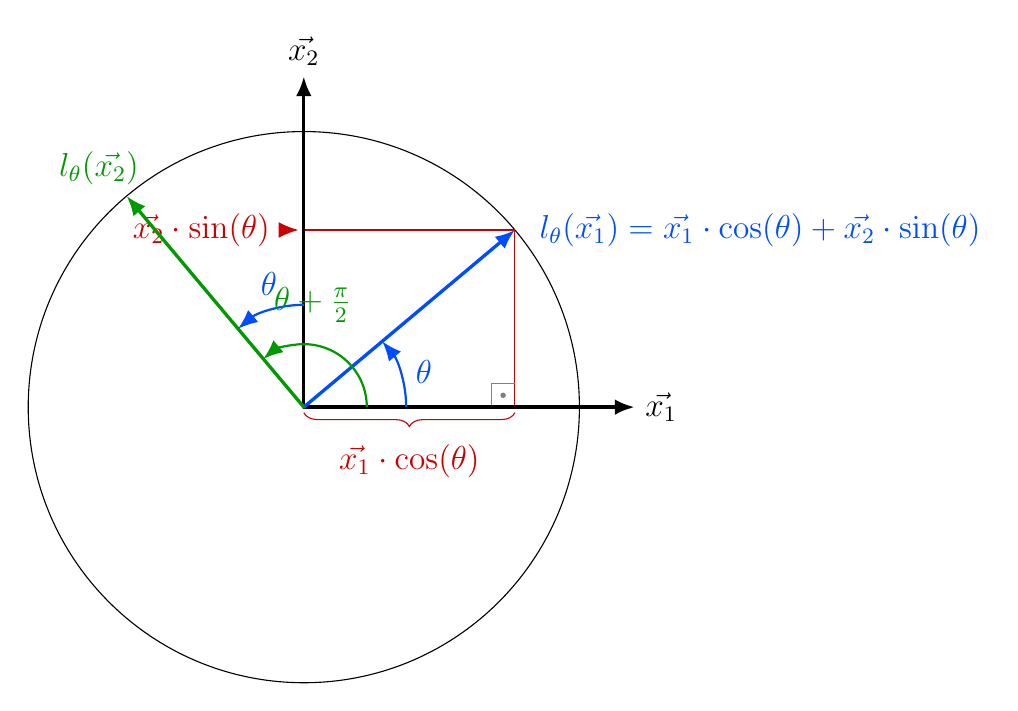
\begin{tikzpicture}[
    thick,
    >={Latex[length=2.5mm, width=2mm]},
    vector/.style={->, very thick, line cap=round},
    basis vector/.style={vector, color=black},
    rotated vector 1/.style={vector, color=blue!70!cyan},
    rotated vector 2/.style={vector, color=green!60!black},
    projection/.style={thin, color=red!80!black},
    angle arc/.style={->, thick},
    every node/.style={font=\large}
]

    % === Parameters ===
    \def\R{3.5} % Radius of the circle
    \def\vlen{4.2} % Length of basis vectors for drawing
    \def\angleval{40} % Angle value for drawing calculations (not shown in text)

    % === Coordinates ===
    \coordinate (O) at (0,0);
    \coordinate (X1_tip) at (\vlen, 0);
    \coordinate (X2_tip) at (0, \vlen);
    \coordinate (LX1) at (\angleval:\R);
    \coordinate (LX2) at (90+\angleval:\R);

    % === Circle ===
    \draw[thin] (O) circle (\R);

    % === Projections of l_theta(x1) ===
    \coordinate (LX1_x) at ({\R*cos(\angleval)}, 0);
    \coordinate (LX1_y) at (0, {\R*sin(\angleval)});

    % Draw projection lines (rectangle)
    \draw[projection] (LX1) -- (LX1_x);
    \draw[projection] (LX1) -- (LX1_y);
    % Draw the components on the axes
    \draw[projection] (O) -- (LX1_x);
    \draw[projection] (O) -- (LX1_y);

    % Curly brace and label for x-component
    \draw[projection, decorate, decoration={brace, amplitude=5pt, mirror, raise=2pt}]
        (O) -- (LX1_x) node[midway, below=10pt] {$\vec{x_1} \cdot \cos(\theta)$};

    % Label for y-component with arrow pointing to the projection on y-axis
    \node[anchor=east, color=red!80!black] (yc_label) at (-0.3, {\R*sin(\angleval)}) {$\vec{x_2} \cdot \sin(\theta)$};
    \draw[->, thin, red!80!black, shorten >=2pt] (yc_label.east) -- (LX1_y);
    
    % Right angle symbol for the projection (gray dot)
    \draw[thin, gray] ($(LX1_x)+(-0.3,0)$) -- ($(LX1_x)+(-0.3,0.3)$) -- ($(LX1_x)+(0,0.3)$);
    \fill[gray] ($(LX1_x)+(-0.15,0.15)$) circle (1pt);


    % === Basis Vectors ===
    \draw[basis vector] (O) -- (X1_tip) node[right] {$\vec{x_1}$};
    \draw[basis vector] (O) -- (X2_tip) node[above] {$\vec{x_2}$};

    % === Rotated Vectors ===
    % l_theta(x1) (blue)
    \draw[rotated vector 1] (O) -- (LX1)
        node[right, xshift=5pt, align=left]
        {$l_\theta(\vec{x_1}) = \vec{x_1} \cdot \cos(\theta) + \vec{x_2} \cdot \sin(\theta)$};

    % l_theta(x2) (green)
    \draw[rotated vector 2] (O) -- (LX2) node[above, xshift=-10pt] {$l_\theta(\vec{x_2})$};


    % === Angles ===
    % Theta for x1 (blue)
    \draw[angle arc, color=blue!70!cyan] (1.3,0) arc (0:\angleval:1.3) node[midway, right, xshift=2pt] {$\theta$};

    % Theta for x2 (red/blue in logic, explicitly labeled theta)
    \draw[angle arc, color=blue!70!cyan] (0,1.3) arc (90:90+\angleval:1.3) node[midway, above, yshift=2pt] {$\theta$};

    % Theta + pi/2 (green)
    \draw[angle arc, color=green!60!black] (0.8,0) arc (0:90+\angleval:0.8);
    \node[color=green!60!black] at (45+\angleval:1.3) {$\theta + \frac{\pi}{2}$};

\end{tikzpicture}
\end{document}
